% mrv-tests.tex

%-------------------------------------------------------------------------
\section{Rappels de cours}\label{tests:cours}
%-------------------------------------------------------------------------
\begin{figure}[ht]
$$\includegraphics[width=10cm]{fig/uml0.pdf}$$
\caption{Flux séquentiel d'instructions}
\label{figure:uml:sequence}
\end{figure}

Sauf mention explicite, les instructions d'un algorithme s'exécutent 
les unes après les autres, dans l'ordre où elles ont été écrites.
Le « chemin » suivi à travers un algorithme est appelé le flux d'instructions
(Figure \ref{figure:uml:sequence}), 
et les constructions qui le modifient sont appelées des instructions de contrôle de flux.
On exécute normalement les instructions de la première à la dernière, sauf lorsqu'on rencontre
une instruction de contrôle de flux : de telles instructions vont permettre de suivre 
différents chemins suivant les circonstances.
C'est en particulier le cas de l'instruction conditionnelle qui n'exécute une instruction
que sous certaines conditions préalables. On distingue ici 3 variantes d'instructions conditionnelles 
(Table \ref{table:python:tests}) : 

\begin{table}[ht]
$$\begin{tabular}{|l|l|}
\hline
\multicolumn{2}{|c|}{\textbf{instructions conditionnelles}}\\
\hline
test simple         & {\begin{minipage}[t]{6cm}\tt if condition : blocIf \\ \mbox{} \end{minipage}} \\
\hline
alternative simple   & {\begin{minipage}[t]{6cm}\tt if condition : blocIf\\else: blocElse \\ \mbox{} \end{minipage}} \\
\hline
alternative multiple & {\begin{minipage}[t]{6cm}\tt if condition : blocIf\\elif condition1: blocElif1\\elif
condition2: blocElif2\\ \ldots \\else: blocElse \\ \mbox{} \end{minipage}}\\
\hline
\multicolumn{2}{p{10cm}}{où {\tt if}, {\tt else} et {\tt elif} sont des mots réservés, {\tt condition} une expression
booléenne (à valeur {\tt True} ou {\tt False}) et {\tt bloc...} un bloc d'instructions.
}
\end{tabular}$$
\caption{Instructions conditionnelles en \python}
\label{table:python:tests}
\end{table}

%-------------------------------------------------------------------------
\subsection{Test simple}\label{tests:cours:test-simple}
%-------------------------------------------------------------------------
L'instruction « {\tt if} » sous sa forme la plus simple
permet de tester la validité d'une condition.
Si la condition est vraie,
alors le bloc d'instructions {\tt blocIf} après le « {\tt :} » est exécuté. 
Si la condition est fausse, on passe à l'instruction suivante dans le flux 
d'instructions. 

\begin{definition}[test simple]
Le test simple est une instruction de contrôle du flux d'instructions 
qui permet d'exécuter une instruction sous condition préalable.
\end{definition}

La condition évaluée après l'instruction « {\tt if} »  est donc une 
expression booléenne qui prend soit la valeur {\tt False} (faux) soit la valeur 
{\tt True} (vrai). Elle peut contenir les opérateurs de comparaison suivants 
(Table \ref{table:python:comparaisons}):

\begin{table}[ht]
$$\begin{tabular}{|l|l|}
\hline
\multicolumn{2}{|c|}{\textbf{opérateurs de comparaison}}\\
\hline
\tt x == y                &  {\tt x} est   égal à {\tt y} \\
\tt x != y                &  {\tt x} est   différent de {\tt y} \\
\tt x > y                 &  {\tt x} est   plus grand que {\tt y} \\
\tt x < y                 &  {\tt x} est   plus petit que {\tt y} \\
\tt x >= y                &  {\tt x} est   plus grand que, ou égal à {\tt y} \\
\tt x <= y                &  {\tt x} est   plus petit que, ou égal à {\tt y}\\
\hline
\end{tabular}$$
\caption{Opérateurs de comparaison en \python}
\label{table:python:comparaisons}
\end{table}

Mais certains problèmes exigent parfois de formuler des conditions qui ne peuvent pas être exprimées 
sous la forme d'une simple comparaison. Par exemple, la condition $x \in [0,1[$ s'exprime 
par la combinaison de deux conditions $x \geq 0$ et $x < 1$ qui doivent être vérifiées en même temps. 
Pour combiner ces conditions, on utilise les opérateurs logiques {\tt not}, {\tt and} et {\tt or}
(Table \ref{table:python:operateurs-logiques}). 
Ainsi la condition $x \in [0,1[$ pourra s'écrire en \python\ :
{\tt (x >= 0) and (x < 1)}.

\begin{table}[ht]
$$\begin{tabular}{|c|c|c|}
\hline
\multicolumn{3}{|c|}{\textbf{opérateurs booléens}}\\
\hline
négation & disjonction & conjonction \\
\hline
\tt not a & \tt a or b & \tt a and b\\
$\begin{array}{|c|c|}
\hline
a & {\overline{a}}\\
\hline
0 & 1\\
1 & 0\\
\hline
\end{array}$ &
$\begin{array}{|c|c|c|}
\hline
a & b & {a+b}\\
\hline
0 & 0 & 0\\
0 & 1 & 1\\
1 & 0 & 1\\
1 & 1 & 1\\
\hline
\end{array}$ &
$\begin{array}{|c|c|c|}
\hline
a & b & {a\cdot b}\\
\hline
0 & 0 & 0\\
0 & 1 & 0\\
1 & 0 & 0\\
1 & 1 & 1\\
\hline
\end{array}$ \\
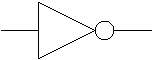
\includegraphics[height=0.75cm]{fig/non.pdf} & 
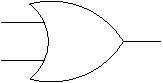
\includegraphics[height=0.75cm]{fig/ou.pdf}  &
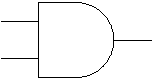
\includegraphics[height=0.75cm]{fig/et.pdf}  \\
\hline
 & \tt not (a or b) & \tt not (a and b) \\
 & 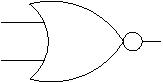
\includegraphics[height=0.75cm]{fig/nonOu.pdf} & \includegraphics[height=0.75cm]{fig/nonEt.pdf}\\
\hline
\end{tabular}
\hfill
\begin{tabular}{ll}
\multicolumn{2}{l}{$\forall a, b, c \in \{0;1\}$ :}\\
\makebox[0.5cm]{} & {$a + 0 = a$} \hspace*{5mm} {$a \cdot 1 = a$}\\
 & {$a + 1 = 1$} \hspace*{5mm} {$a \cdot 0 = 0$}\\
 & {$a + a = a$} \hspace*{5mm} {$a \cdot a = a$}\\
 & {$a + \overline{a} = 1$} \hspace*{5mm} {$a \cdot \overline{a} = 0$}\\
 & {$a + (a \cdot b) = a$} \hspace*{5mm} {$a \cdot (a + b) = a$}\\
 & {$\overline{\overline{a}}  = a$} \hspace*{5mm} $\overline{a + b} = \overline{a} \cdot \overline{b}$ \hspace*{5mm} $\overline{a\cdot b} = \overline{a} + \overline{b}$\\
 & {$(a+b) = (b+a)$} \hspace*{5mm}  {$(a \cdot b) = (b \cdot a)$} \\
 & {$(a+b)+c = a+(b+c)$} \\ 
 & {$(a\cdot b)\cdot c = a\cdot (b\cdot c)$} \\
 & {$a + (b \cdot c) = (a+b) \cdot (a+c)$} \\ 
 & {$a \cdot (b+ c) = (a \cdot b)+(a\cdot c)$} 
\end{tabular}$$
\caption{Opérateurs logiques en \python}
\label{table:python:operateurs-logiques}
\end{table}

%-------------------------------------------------------------------------
\subsection{Alternative simple}\label{tests:cours:alternative-simple}
%-------------------------------------------------------------------------

L'instruction « {\tt if} \ldots\ {\tt else} » teste une condition. 
Si la condition
est vraie, alors le bloc d'instructions {\tt blocIf} après le « {\tt :} » est exécuté.
Si la condition est fausse, c'est le bloc d'instructions {\tt blocElse} après le « {\tt else:} » 
(sinon) qui est exécuté. Seul l'un des 2 blocs est donc exécuté.

\begin{definition}[alternative simple]
L'alternative simple est une instruction de contrôle du flux d'instructions 
qui permet de choisir entre deux instructions selon qu'une condition est vérifiée ou non.
\end{definition}

La figure \ref{figure:uml:alternative-simple} montre
qu'une alternative se comporte comme un aiguillage de chemin de fer 
dans le flux d'instructions. 
Un « {\tt if ... else} » ouvre  deux voies correspondant à deux traitements différents, 
et seule une de ces voies sera empruntée (un seul des deux traitements est
exécuté). 
A ce titre, le test simple de la section \ref{tests:cours:test-simple} précédente est équivalent 
à une alternative simple où on explicite le fait de ne rien faire (instruction {\tt pass})
dans le bloc d'instructions associé au {\tt else}.

\begin{figure}[ht]
$$\begin{minipage}{10cm}
\begin{Verbatim}
if condition : blocIf
else         : blocElse
\end{Verbatim}
\end{minipage}$$
$${\includegraphics[width=10cm]{fig/uml1.pdf}}$$
$$\begin{minipage}{10cm}
L'étiquette {\tt [condition]} signifie qu'on passe par la voie correspondante 
si la condition est vérifiée ({\tt True}), sinon on passe par la voie étiquettée
{\tt [else]}.
\end{minipage}$$
\caption{Alternative simple en \python}
\label{figure:uml:alternative-simple}
\end{figure}

Mais il y a des situations où deux voies ne suffisent pas : on utilise
alors des alternatives simples en cascade (ou alternatives multiples). 

%-------------------------------------------------------------------------
\subsection{Alternative multiple}\label{tests:cours:alternative-multiple}
%-------------------------------------------------------------------------

L'instruction « {\tt if} \ldots\ {\tt elif} » teste une première condition. 
Si cette condition est vraie, alors le bloc d'instructions {\tt blocIf} 
est exécuté. Si la première condition est fausse, on teste la deuxième ({\tt condition1}).
Si la deuxième condition est vérifiée, c'est le bloc d'instructions {\tt blocElif1} après le premier « {\tt elif:} » 
(sinon-si) qui est exécuté; sinon on teste la condition suivante ({\tt condition2}).
Si elle est vérifiée, c'est le bloc d'instructions {\tt blocElif2} après le deuxième « {\tt elif:} » 
qui est exécuté et ainsi de suite. Si aucune des conditions n'est vérifiée, c'est le bloc d'instructions
{\tt blocElse} qui est exécuté. Dans tous les cas, un seul des blocs est donc exécuté.

\begin{definition}[alternative multiple]
L'alternative multiple est une instruction de contrôle du flux d'instructions 
qui permet de choisir entre plusieurs instructions en cascadant des alternatives simples.
\end{definition}

%-------------------------------------------------------------------------
\section{Vie courante : mention au baccalauréat}\label{tests:vie-courante}
%-------------------------------------------------------------------------

\subsection{Objectif}\label{tests:vie-courante:objectif}
\begin{description}
\item[Principal : ] mettre en \oe uvre l'instruction d'alternative multiple.
\item[Secondaire :] déterminer la mention au bac.
\end{description}

\subsection{Syntaxe \python}\label{tests:vie-courante:python}
\noindent\begin{minipage}[t]{0.3\textwidth}
test simple\footnotesize
\begin{Verbatim}
if condition : bloc
\end{Verbatim}
\end{minipage}
\hfill
\begin{minipage}[t]{0.3\textwidth}
alternative simple\footnotesize
\begin{Verbatim}
if condition : bloc1
else         : bloc2
\end{Verbatim}
\end{minipage}
\hfill
\begin{minipage}[t]{0.3\textwidth}
alternative multiple\footnotesize
\begin{Verbatim}
if   condition1 : bloc1
elif condition2 : bloc2
elif condition3 : bloc3
...
else            : blocn
\end{Verbatim}
\end{minipage}

\subsection{Enoncé}\label{tests:vie-courante:enonce}

\subsection{Méthode}\label{tests:vie-courante:methode}

\subsection{Résultat}\label{tests:vie-courante:resultat}

\subsection{Vérification}\label{tests:vie-courante:verification}

\subsection{Généricité}\label{tests:vie-courante:genericite}

\subsection{Entraînement}\label{tests:vie-courante:entrainement}

%-------------------------------------------------------------------------
\section{Jeux : 421}
%-------------------------------------------------------------------------

\subsection{Objectif}\label{tests:jeux:objectif}
\begin{description}
\item[Principal : ] mettre en \oe uvre l'instruction d'alternative multiple.
\item[Secondaire :] .
\end{description}

\subsection{Syntaxe \python}\label{tests:jeux:python}
\noindent\begin{minipage}[t]{0.3\textwidth}
test simple\footnotesize
\begin{Verbatim}
if condition : bloc
\end{Verbatim}
\end{minipage}
\hfill
\begin{minipage}[t]{0.3\textwidth}
alternative simple\footnotesize
\begin{Verbatim}
if condition : bloc1
else         : bloc2
\end{Verbatim}
\end{minipage}
\hfill
\begin{minipage}[t]{0.3\textwidth}
alternative multiple\footnotesize
\begin{Verbatim}
if   condition1 : bloc1
elif condition2 : bloc2
elif condition3 : bloc3
...
else            : blocn
\end{Verbatim}
\end{minipage}

\subsection{Enoncé}\label{tests:jeux:enonce}

\subsection{Méthode}\label{tests:jeux:methode}

\subsection{Résultat}\label{tests:jeux:resultat}

\subsection{Vérification}\label{tests:jeux:verification}

\subsection{Généricité}\label{tests:jeux:genericite}

\subsection{Entraînement}\label{tests:jeux:entrainement}


%-------------------------------------------------------------------------
\section{Textes : }
%-------------------------------------------------------------------------

\subsection{Objectif}\label{tests:textes:objectif}
Mettre en \oe uvre l'instruction d'alternative multiple sur un exemple de type « textes ».

\subsection{Syntaxe \python}\label{tests:textes:python}
\noindent\begin{minipage}[t]{0.3\textwidth}
test simple\footnotesize
\begin{Verbatim}
if condition : bloc
\end{Verbatim}
\end{minipage}
\hfill
\begin{minipage}[t]{0.3\textwidth}
alternative simple\footnotesize
\begin{Verbatim}
if condition : bloc1
else         : bloc2
\end{Verbatim}
\end{minipage}
\hfill
\begin{minipage}[t]{0.3\textwidth}
alternative multiple\footnotesize
\begin{Verbatim}
if   condition1 : bloc1
elif condition2 : bloc2
elif condition3 : bloc3
...
else            : blocn
\end{Verbatim}
\end{minipage}

\subsection{Enoncé}\label{tests:textes:enonce}

\subsection{Méthode}\label{tests:textes:methode}

\subsection{Résultat}\label{tests:textes:resultat}

\subsection{Vérification}\label{tests:textes:verification}

\subsection{Généricité}\label{tests:textes:genericite}

\subsection{Entraînement}\label{tests:textes:entrainement}

%-------------------------------------------------------------------------
\section{Nombres : }
%-------------------------------------------------------------------------

\subsection{Objectif}\label{tests:nombres:objectif}
\begin{description}
\item[Principal : ] mettre en \oe uvre l'instruction d'alternative multiple.
\item[Secondaire :] .
\end{description}

\subsection{Syntaxe \python}\label{tests:nombres:python}
\noindent\begin{minipage}[t]{0.3\textwidth}
test simple\footnotesize
\begin{Verbatim}
if condition : bloc
\end{Verbatim}
\end{minipage}
\hfill
\begin{minipage}[t]{0.3\textwidth}
alternative simple\footnotesize
\begin{Verbatim}
if condition : bloc1
else         : bloc2
\end{Verbatim}
\end{minipage}
\hfill
\begin{minipage}[t]{0.3\textwidth}
alternative multiple\footnotesize
\begin{Verbatim}
if   condition1 : bloc1
elif condition2 : bloc2
elif condition3 : bloc3
...
else            : blocn
\end{Verbatim}
\end{minipage}

\subsection{Enoncé}\label{tests:nombres:enonce}

\subsection{Méthode}\label{tests:nombres:methode}

\subsection{Résultat}\label{tests:nombres:resultat}

\subsection{Vérification}\label{tests:nombres:verification}

\subsection{Généricité}\label{tests:nombres:genericite}

\subsection{Entraînement}\label{tests:nombres:entrainement}

%-------------------------------------------------------------------------
\section{Figures : }
%-------------------------------------------------------------------------

\subsection{Objectif}\label{tests:figures:objectif}
\begin{description}
\item[Principal : ] mettre en \oe uvre l'instruction d'alternative multiple.
\item[Secondaire :] .
\end{description}

\subsection{Syntaxe \python}\label{tests:figures:python}
\noindent\begin{minipage}[t]{0.3\textwidth}
test simple\footnotesize
\begin{Verbatim}
if condition : bloc
\end{Verbatim}
\end{minipage}
\hfill
\begin{minipage}[t]{0.3\textwidth}
alternative simple\footnotesize
\begin{Verbatim}
if condition : bloc1
else         : bloc2
\end{Verbatim}
\end{minipage}
\hfill
\begin{minipage}[t]{0.3\textwidth}
alternative multiple\footnotesize
\begin{Verbatim}
if   condition1 : bloc1
elif condition2 : bloc2
elif condition3 : bloc3
...
else            : blocn
\end{Verbatim}
\end{minipage}

\subsection{Enoncé}\label{tests:figures:enonce}

\subsection{Méthode}\label{tests:figures:methode}

\subsection{Résultat}\label{tests:figures:resultat}

\subsection{Vérification}\label{tests:figures:verification}

\subsection{Généricité}\label{tests:figures:genericite}

\subsection{Entraînement}\label{tests:figures:entrainement}

%-------------------------------------------------------------------------
\section{Mathématiques : graphe de fonction}
%-------------------------------------------------------------------------

\subsection{Objectif}\label{tests:maths:objectif}
\begin{description}
\item[Principal : ] mettre en \oe uvre l'instruction d'alternative multiple.
\item[Secondaire :] .
\end{description}

\subsection{Syntaxe \python}\label{tests:maths:python}
\noindent\begin{minipage}[t]{0.3\textwidth}
test simple\footnotesize
\begin{Verbatim}
if condition : bloc
\end{Verbatim}
\end{minipage}
\hfill
\begin{minipage}[t]{0.3\textwidth}
alternative simple\footnotesize
\begin{Verbatim}
if condition : bloc1
else         : bloc2
\end{Verbatim}
\end{minipage}
\hfill
\begin{minipage}[t]{0.3\textwidth}
alternative multiple\footnotesize
\begin{Verbatim}
if   condition1 : bloc1
elif condition2 : bloc2
elif condition3 : bloc3
...
else            : blocn
\end{Verbatim}
\end{minipage}

\subsection{Enoncé}\label{tests:maths:enonce}
On considère dans $\mathbb{R}$ la fonction continue $f$, affine par morceaux,  
définie sur $[-5;5]$  par le graphe ci-dessous et $\forall x < -5, f(x) = f(-5)$
et $\forall x > 5, f(x) = f(5)$. 
$$%\begin{minipage}{6.75cm}
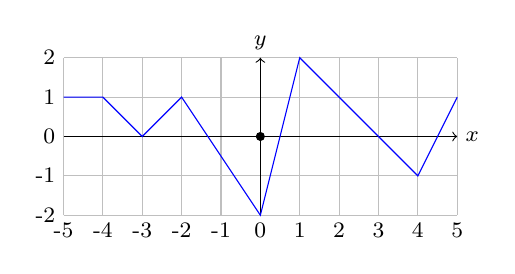
\begin{tikzpicture}[scale=0.5]\footnotesize
\draw[color=lightgray](-5,-2) grid[xstep=1,ystep=1] (5,2);
\foreach \x in {-5,-4,...,5} \draw(\x,-2) node[below]{\x};
\foreach \y in {-2,-1,...,2} \draw(-5,\y) node[left]{\y};
\filldraw(0,0) circle (0.1);
\draw[->] (-5,0) -- (5,0);
\draw (5,0) node[right]{$x$} ;
\draw[->] (0,-2) -- (0,2);
\draw (0,2) node[above]{$y$};
\draw[color=blue] (-5,1) -- (-4,1) -- (-3,0) -- (-2,1) -- (0,-2) -- (1,2) -- (4,-1) -- (5,1);
%\draw (-4.5,1) node[above]{\Pisymbol{pzd}{172}};
%\draw (-3.5,0.5) node[above]{\Pisymbol{pzd}{173}};
%\draw (-2.5,0.5) node[below]{\Pisymbol{pzd}{174}};
%\draw (-1,-0.5) node[below]{\Pisymbol{pzd}{175}};
%\draw (0.5,0) node[right]{\Pisymbol{pzd}{176}};
%\draw (2.5,0.5) node[right]{\Pisymbol{pzd}{177}};
%\draw (4.5,0) node[above]{\Pisymbol{pzd}{178}};
\end{tikzpicture}
%\end{minipage}
$$
Proposer une instruction de type « alternative multiple » qui permettra de calculer 
la fonction $y = f(x)$ $\forall x \in \mathbb{R}$.

\subsection{Méthode}\label{tests:maths:methode}
Il s'agit de déterminer la valeur $y = f(x)$ d'une fonction continue affine par morceaux sur $\mathbb{R}$. L'axe des réels $]-\infty,x_1,x_2,\ldots,x_n,+\infty[$ est donc vu comme une
succession d'intervalles $]-\infty,x_1[$, $[x_1,x_2[$, \ldots, $[x_{n-1},x_n[$ et
$[x_n,+\infty[$ sur lesquels la fonction $f$ est définie respectivement par les fonctions $f_1$, $f_2$, \ldots, $f_n$ et $f_{n+1}$ :
$$\begin{tabular}{l@{ $=$ }l@{ $\forall x \in$ }l}
$y = f(x)$ 	& $f_1(x)$		& $]-\infty,x_1[$ \\
			& $f_2(x)$ 		& $[x_1,x_2[$ \\
			& $f_3(x)$ 		& $[x_2,x_3[$ \\
			& \multicolumn{2}{l}{\ldots} \\
			& $f_n(x)$ 		& $[x_{n-1},x_n[$\\
			& $f_{n+1}(x)$ 	& $[x_n,+\infty[$
\end{tabular}$$
Chacune des fonctions $f_i$ correspond à une droite d'équation $y = a_ix+b_i$ où $a_i$
représente la pente de la droite et $b_i$ son ordonnée à l'origine.
Lorsqu'on connaît 2 points $M(x_M,y_M)$ et $N(x_N,y_N)$ 
d'une droite d'équation $y = ax + b$, les coefficients $a$ (pente de la droite) 
et $b$ (ordonnée à l'origine) de la droite sont obtenus
par résolution du système de 2 équations : $y_M =ax_M + b$ et $y_N = ax_N + b$. 
On obtient alors $a$ et $b$ :

$$\begin{minipage}{6.75cm}
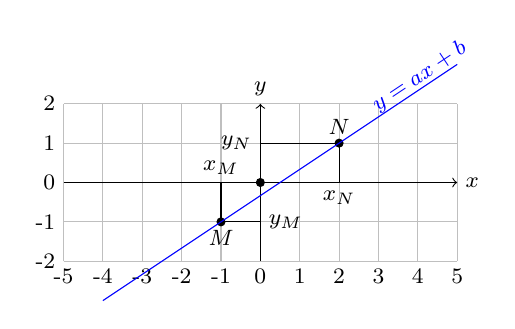
\begin{tikzpicture}[scale=0.5]\footnotesize
\draw[color=lightgray](-5,-2) grid[xstep=1,ystep=1] (5,2);
\foreach \x in {-5,-4,...,5} \draw(\x,-2) node[below]{\x};
\foreach \y in {-2,-1,...,2} \draw(-5,\y) node[left]{\y};
\filldraw(0,0) circle (0.1);
\filldraw(-1,-1) circle (0.1);
\draw (-1,-1) node[below]{$M$};
\draw(-1,0) node[above]{$x_M$};
\draw(0,-1) node[right]{$y_M$};
\draw (-1,-1) -- (-1,0);
\draw (-1,-1) -- (0,-1);
\filldraw(2,1) circle (0.1);
\draw (2,1) node[above]{$N$};
\draw(2,0) node[below]{$x_N$};
\draw(0,1) node[left]{$y_N$};
\draw (2,1) -- (2,0);
\draw (2,1) -- (0,1);
\draw[->] (-5,0) -- (5,0);
\draw (5,0) node[right]{$x$} ;
\draw[->] (0,-2) -- (0,2);
\draw (0,2) node[above]{$y$};
\draw[color=blue] (-4,-3) -- (5,3);
\draw[color=blue](4.3,2.3) node[above,rotate=33.69]{$y = ax + b$};
\end{tikzpicture}
\end{minipage}
\hfill
\begin{minipage}{8.75cm}
$$\displaystyle a = \frac{y_N - y_M}{x_N - x_M} \mbox{ et } \displaystyle b = \frac{y_Mx_N - y_Nx_M}{x_N - x_M}$$
Pour la droite ci-contre :
$$\displaystyle 
a = \frac{1 - (-1)}{2 - (-1)} = \frac{2}{3} \mbox{ et } \displaystyle 
b = \frac{(-1)\cdot 2 - 1\cdot(-1)}{2 - (-1)} = -\frac{1}{3}
$$
On vérifie graphiquement ces résultats : pour passer de $M$ à $N$, on
se déplace de $\Delta x = 3$ horizontalement puis de $\Delta y = 2$ verticalement 
(d'où la pente $a = \Delta y/\Delta x = 2/3$),
et la droite coupe bien l'axe des ordonnées en $y = -1/3$.
\end{minipage}$$
Une fois déterminés les coefficients $a_i$ et $b_i$ de chaque droite, on détermine
la valeur de la fonction $y = f(x)$ par une alternative multiple du genre :
$$\begin{minipage}{5.5cm}\tt
if   x < $x_1$ : y = $a_1$*x + $b_1$\\
elif x < $x_2$ : y = $a_2$*x + $b_2$\\
elif x < $x_3$ : y = $a_3$*x + $b_3$\\
...\\
elif x < $x_n$ : y = $a_n$*x + $b_n$\\
else           : y = $a_{n+1}$*x + $b_{n+1}$
\end{minipage}$$

\subsection{Résultat}\label{tests:maths:resultat}
On applique la méthode précédente à la fonction $f$ de l'énoncé.
Il faut donc déterminer les équations de droite 
correspondant aux différents segments du graphe de la fonction, à savoir :
$$\begin{minipage}{9cm}
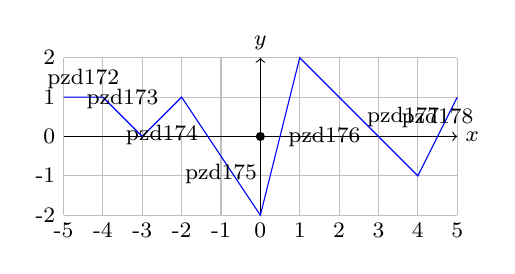
\begin{tikzpicture}[scale=0.5]\footnotesize
\draw[color=lightgray](-5,-2) grid[xstep=1,ystep=1] (5,2);
\foreach \x in {-5,-4,...,5} \draw(\x,-2) node[below]{\x};
\foreach \y in {-2,-1,...,2} \draw(-5,\y) node[left]{\y};
\filldraw(0,0) circle (0.1);
\draw[->] (-5,0) -- (5,0);
\draw (5,0) node[right]{$x$} ;
\draw[->] (0,-2) -- (0,2);
\draw (0,2) node[above]{$y$};
\draw[color=blue] (-5,1) -- (-4,1) -- (-3,0) -- (-2,1) -- (0,-2) -- (1,2) -- (4,-1) -- (5,1);
\draw (-4.5,1) node[above]{\Pisymbol{pzd}{172}};
\draw (-3.5,0.5) node[above]{\Pisymbol{pzd}{173}};
\draw (-2.5,0.5) node[below]{\Pisymbol{pzd}{174}};
\draw (-1,-0.5) node[below]{\Pisymbol{pzd}{175}};
\draw (0.5,0) node[right]{\Pisymbol{pzd}{176}};
\draw (2.5,0.5) node[right]{\Pisymbol{pzd}{177}};
\draw (4.5,0) node[above]{\Pisymbol{pzd}{178}};
\end{tikzpicture}
\end{minipage}
\hfill
\begin{minipage}{3cm}
\begin{itemize}
\item[\Pisymbol{pzd}{172}] $y = 1$
\item[\Pisymbol{pzd}{173}] $y = -x -3$
\item[\Pisymbol{pzd}{174}] $y = x + 3$
\item[\Pisymbol{pzd}{175}] $y = -3x/2 - 2$
\item[\Pisymbol{pzd}{176}] $y = 4x - 2$
\item[\Pisymbol{pzd}{177}] $y = -x + 3$
\item[\Pisymbol{pzd}{178}] $y = 2x - 9$
\end{itemize}
\end{minipage}$$

\noindent\begin{minipage}[t]{7cm}
Compte-tenu de ces équations, le code ci-contre
permet de calculer $y = f(x)$, y compris pour $x < -5$ ($y = f(-5) =1$) et 
$x > 5$ ($y = f(5) = 1$).

Remarque : on aurait pu simplifier les deux premières lignes de ce code en\\
\centerline{\texttt{if x < -4 : y = 1}}
car les instructions associées sont iden\-tiques (ie. les fonctions
affines sont identiques sur $]-\infty,-5[$ et $[-5,-4[$).
\end{minipage}
\hfill
\begin{minipage}[t]{8cm}\footnotesize
\begin{lstlisting}[caption=\textbf{graphe d'une fonction}]
if   x < -5 : y = 1
elif x < -4 : y = 1
elif x < -3 : y = -x - 3
elif x < -2 : y = x + 3
elif x <  0 : y = -3*x/2 - 2
elif x <  1 : y = 4*x - 2
elif x <  4 : y = -x + 3
elif x <  5 : y = 2*x - 9
else        : y = 1
\end{lstlisting}
\end{minipage}

\subsection{Vérification}\label{tests:maths:verification}
Pour tester le résultat précédent, 
on peut comparer les valeurs obtenues par le calcul avec celles lues
directement sur le graphe pour quelques points caractéristiques.
Ces points de mesure sont choisis judicieusement : ils ne correspondent 
pas aux bornes des intervalles déjà prises en compte dans la méthode
mais plutôt à des points où la fonction s'annule 
(exemples : $x = -4/3$, $1/2$, $3$ ou $9/2$)
ou à des points d'abscisses aux n\oe uds de la grille de lecture 
(exemples : $x = -1$ ou $x = 2$).
On peut vérifier par exemple pour $x = -1$ 
($y = f(-1) = -1/2$) et $x = 3$ ($y = f(3) = 0$).
$$\begin{minipage}{7.5cm}\footnotesize
\begin{Verbatim}
>>> x = -1
>>> if x < -4 : y = 1
elif   x < -3 : y = -x - 3
elif   x < -2 : y = x + 3
elif   x <  0 : y = -3*x/2 - 2
elif   x <  1 : y = 4*x - 2
elif   x <  4 : y = -x + 3
elif   x <  5 : y = 2*x - 9
else          : y = 1

>>> y
-0.5
\end{Verbatim}
\end{minipage}
\hfill
\begin{minipage}{7.5cm}\footnotesize
\begin{Verbatim}
>>> x = 3
>>> if x < -4 : y = 1
elif   x < -3 : y = -x - 3
elif   x < -2 : y = x + 3
elif   x <  0 : y = -3*x/2 - 2
elif   x <  1 : y = 4*x - 2
elif   x <  4 : y = -x + 3
elif   x <  5 : y = 2*x - 9
else          : y = 1

>>> y
0
\end{Verbatim}
\end{minipage}$$
On obtient bien par le calcul les résultats lus sur la grille.

\subsection{Généricité}\label{tests:maths:genericite}
Pour vérifier la généricité de la méthode précédente,
proposer une alternative multiple pour chacune des 2 fonctions définies sur $[-5;5]$ 
par les graphes ci-dessous et $\forall x <~-5, f(x) = f(-5)$
et $\forall x > 5, f(x) = f(5)$.

\begin{minipage}{7cm}
\begin{enumerate}
\item 
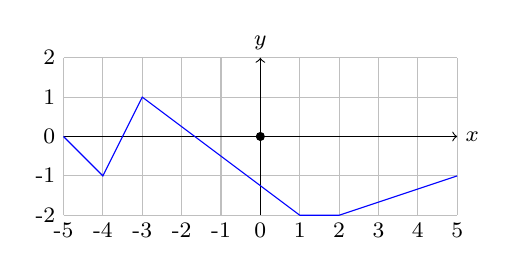
\begin{tikzpicture}[scale=0.5]\footnotesize
\draw[color=lightgray](-5,-2) grid[xstep=1,ystep=1] (5,2);
\foreach \x in {-5,-4,...,5} \draw(\x,-2) node[below]{\x};
\foreach \y in {-2,-1,...,2} \draw(-5,\y) node[left]{\y};
\filldraw(0,0) circle (0.1);
\draw[->] (-5,0) -- (5,0); 
\draw (5,0) node[right]{$x$} ;
\draw[->] (0,-2) -- (0,2);
\draw (0,2) node[above]{$y$};
\draw[color=blue] (-5,0) -- (-4,-1) -- (-3,1) -- (1,-2) -- (2,-2) -- (5,-1);
\end{tikzpicture}
\end{enumerate}
\end{minipage}
\hfill
\begin{minipage}{7cm}
\begin{enumerate}\setcounter{enumi}{1}
\item 
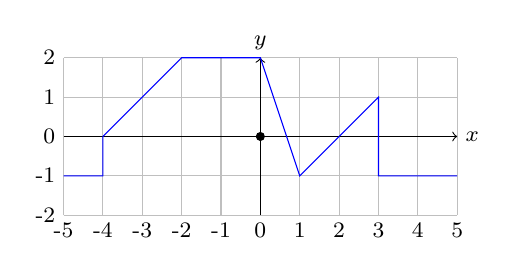
\begin{tikzpicture}[scale=0.5]\footnotesize
\draw[color=lightgray](-5,-2) grid[xstep=1,ystep=1] (5,2);
\foreach \x in {-5,-4,...,5} \draw(\x,-2) node[below]{\x};
\foreach \y in {-2,-1,...,2} \draw(-5,\y) node[left]{\y};
\filldraw(0,0) circle (0.1);
\draw[->] (-5,0) -- (5,0);
\draw (5,0) node[right]{$x$} ;
\draw[->] (0,-2) -- (0,2);
\draw (0,2) node[above]{$y$};
\draw[color=blue] (-5,-1) -- (-4,-1) -- (-4,0) -- (-2,2) -- (0,2) -- (1,-1) -- (1,-1) -- (3,1) -- (3,-1) -- (5,-1);
\end{tikzpicture}
\end{enumerate}
\end{minipage}

\subsection{Entraînement}\label{tests:maths:entrainement}
Utiliser une alternative multiple pour déterminer les racines réelles
d'un trinôme du second degré $ax^2 + bx + c$ à coefficients $a$, $b$ et $c$ réels.


%-------------------------------------------------------------------------
\section{Physique : états de l'eau}
%-------------------------------------------------------------------------

\subsection{Objectif}\label{tests:physique:objectif}
\begin{description}
\item[Principal : ] mettre en \oe uvre l'instruction d'alternative multiple.
\item[Secondaire :] .
\end{description}

\subsection{Syntaxe \python}\label{tests:physique:python}

\subsection{Enoncé}\label{tests:physique:enonce}


\subsection{Méthode}\label{tests:physique:methode}

\subsection{Résultat}\label{tests:physique:resultat}

\subsection{Vérification}\label{tests:physique:verification}

\subsection{Généricité}\label{tests:physique:genericite}

\subsection{Entraînement}\label{tests:physique:entrainement}

%-------------------------------------------------------------------------
\section{Informatique : }
%-------------------------------------------------------------------------

\subsection{Objectif}\label{tests:informatique:objectif}
\begin{description}
\item[Principal : ] mettre en \oe uvre l'instruction d'alternative multiple.
\item[Secondaire :] .
\end{description}

\subsection{Syntaxe \python}\label{tests:informatique:python}
\noindent\begin{minipage}[t]{0.3\textwidth}
test simple\footnotesize
\begin{Verbatim}
if condition : bloc
\end{Verbatim}
\end{minipage}
\hfill
\begin{minipage}[t]{0.3\textwidth}
alternative simple\footnotesize
\begin{Verbatim}
if condition : bloc1
else         : bloc2
\end{Verbatim}
\end{minipage}
\hfill
\begin{minipage}[t]{0.3\textwidth}
alternative multiple\footnotesize
\begin{Verbatim}
if   condition1 : bloc1
elif condition2 : bloc2
elif condition3 : bloc3
...
else            : blocn
\end{Verbatim}
\end{minipage}

\subsection{Enoncé}\label{tests:informatique:enonce}

\subsection{Méthode}\label{tests:informatique:methode}

\subsection{Résultat}\label{tests:informatique:resultat}

\subsection{Vérification}\label{tests:informatique:verification}

\subsection{Généricité}\label{tests:informatique:genericite}

\subsection{Entraînement}\label{tests:informatique:entrainement}

%-------------------------------------------------------------------------
\section{Retours d'expériences}\label{tests:retours}
%-------------------------------------------------------------------------

%-------------------------------------------------------------------------
\subsection{Méthode}\label{tests:retours:methode}

%-------------------------------------------------------------------------
\subsection{Résultat}\label{tests:retours:resultat}

%-------------------------------------------------------------------------
\subsection{Vérification}\label{tests:retours:verification}

